\chapter{Αποτελέσματα του STAR}

\section{Συγκρούσεις Βαρέων Ιόντων}

	Η QCD  είναι η θεμελιώδης θεωρία στην οποία βασίζεται η μελέτη των ισχυρών αλληλεπιδράσεων μεταξύ των Κουάρκ και των Γλουονίων και κατ΄επέκταση είναι αυτή που υπαγορεύει την δομή των αδρονίων και των πυρήνων.
	Η 	QCD επιβάλλει πως τα Κουάρκ και τα Γλουόνια είναι περιορισμένα εντός των αδρονίων τα οποία αποτελεούν την μόνη ευσταθή κατάσταση.
	
	Υπό ακραίες συνθήκες υψηλής θερμοκρασίας και πυκνότητας βαρυονίων, προβλέπεται πως συμβαίνει μία αλλαγή φάσης. Κατά αυτή την μετάβαση μπορούν να υπάρξουν ελεύθερα Κουάρκ και Γλουόνια και ονομάζεται, κατά το Ηλεκτρομαγνητικό ανάλογο, Πλάσμα Κουάρκ-Γλουονίων ( Quark-Gluon Plasma, GCP).  
	Αριθμητικές προβλέψεις υποδεικνύουν πως πράγματι συμβαίνει μία σχεδόν πρώτης τάξης αλλαγή φάσης σε μία κρίσιμη θερμοκρασία περίπου 170MeV(~2TeraKelvin).
	Αυτή η κατάσταση εικάζεται πως υπήρχει στα πρώτα κλάσματα του δευτερολέπτου μετά το Big Bang, πως επικρατεί στο εσωτερικό των αστέρων νετρονίων σε συνθήκες πολύ υψηλής πυκνότητας αλλά και πως μπορεί να δημιουργηθεί τεχνητά από συγκρούσεις βαρέων ιόντων.
		
	
	Πριν την κατασκευή του RHIC και των αντίστοιχων ανιχνευτών του, υπήρχαν ήδη άλλα πειράματα όπως το AGS και το SPS κατασκευασμένα την δεκαετία του 80' όπου ένας από τους στόχους τους χρησιμοποιώντας συγκρούσεις βαρέων ιόντων ήταν η εύρεση του QGP. 
	Όπως έχει αναφερθεί, μία από τις κύριες διεργασίες που συμβαίνουν στον RHIC είναι οι συγκρούσεις βαρέων ιόντων και κυρίως Au-Au με ενέργεια έως και $\sqrt{s}=200GeV/n$, δηλαδή συνολική ενέργεια περίπου 32TeV/ion .
	 Από την περίοδο κατασκευής του RHIC περίμεναν να δούν ενδείξεις για την δημιουργία του QGP καθώς η ανίχνευτή του αποτελούσε έναν από τους βασικούς στόχους του.
	Η εξέλιξη των συγκρούσεων βαρέων ιόντων φαίνεται στις Εικόνες (\ref{fig4.1})\&(\ref{fig4.2}). 
	
	\begin{figure}[h!]
	    \centering
	    \begin{minipage}{.5\textwidth}
	        \centering
	        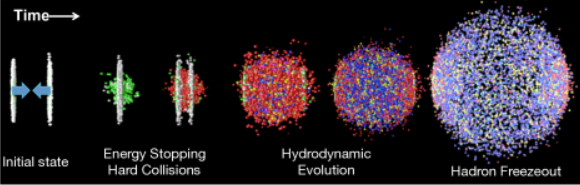
\includegraphics[scale=0.7]{STAR_Results/QGP_formation2}
	        \caption{Εξέλιξη των συγκρούσεων βαρέων ιόντων}
	        \label{fig4.1}
	    \end{minipage}%
	    \begin{minipage}{0.5\textwidth}
	        \centering
	        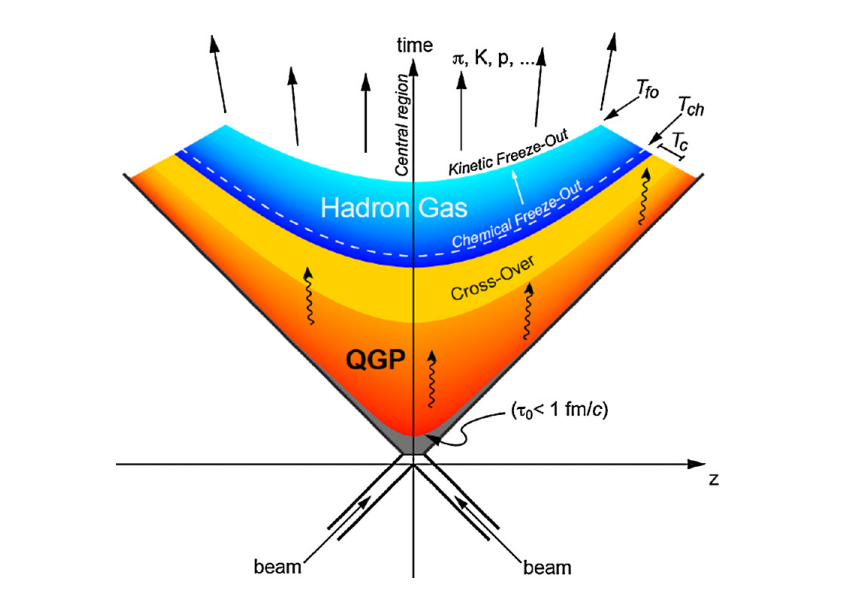
\includegraphics[scale=0.6]{STAR_Results/QGP_time_evolution}
	        \caption{Στάδια μετά την σύγκρουση βαρέων ιόντων}
	        \label{fig4.2}
	    \end{minipage}
	\end{figure}
	
	Πριν περάσουμε σε αποτελέσματα σχετικά με το πείραμα STAR που ένας στόχος του είναι η μελέτη κάποιων χαρακτηριστικών των παραπάνω συγκρούσεων θα πρέπει να δούμε 
πως ακριβώς αυτές εξελίσσονται και έπειτα να ορίσουμε το τί ακριβώς είναι το QGP. 		
	%Το  πρώτο στάδιο μετά την αλληλεπίδραση είναι αποδέσμευση των κουάρκ από τα αδρόνια και η δημιουργία του GQP, εάν βέβεια οι πυρήνες έχουν αρκετά μεγάλη ενέργεια.
	%Έπειτα, το σύστημα διστέλεται, πέφτει η θερμοκρασία του, έρχεται σε θερμική και χημική ισορροπία και ξανασχηματίζονται τα αδρόνια της τελικής κατάσταση τα οποία εν τέλει ανιχνεύουμε. Η χρονική κλίμακα που εξελίσσεται το φαίνόμενο είναι της τάξης $~10^{-23}$sec.
	Το αρχικό στάδιο, $\tau<0$\footnote{$\tau$ είναι ο proper time} είναι πριν την σύγκρουση	 όπου τα κουάρκ και τα γλουόνια υπάρχουν μέσα στα νετρόνια και τα πρωτόνιο με την συνάρτηση δομής τους.
	Μετά την σύγκρουση, για $0<\tau<\tau_0$, έρχεται το στάδιο των παρτονίων όπου η αρχική κινητική ενέργεια εναποτίθεται στην περιοχή επικάλυψης των πυρήνων. Αυτή η ενέργεια παράγει μία διεγερμένη κατάσταση της ύλης που καλείται \textit{fireball}. Αν αυτή η κινητική ενέργεια και η θερμοκρασία είναι αρκετά υψηλές, τότε δημιουργείται η κατάσταση στην οποία τα κουάρκ και τα γλουόνια αποδεσμεύονται από τα νουκλεόνια και φτιάχνουν το QGP.
	Στην συνέχεια, για $\tau_0<\tau<\tau_f$, οι συχνές αλληλεπιδράσεις και συγκρούσεις μεταξύ των συστατικών της \textit{fireball} οδηγούν το σύστημα σε θερμική ισοροπία και ταυτόχρονα λόγω της βαθμίδας της πίεσης σε διαστολή.
	Όσο το σύστημα διαστέλλεται ταυτόχρονα κρυώνει μέχρι να φτάσει σε μία κρίσιμη θερμοκρασία $T_c$, κάτω από την οποία αρχίζει η αδρονοποίηση, δηλαδή μία μετάβαση κατά την οποία τα αποδεσμευμένα κουάρκ και γλουόνια μετασχηματίζονται σε αδρόνια.
	%
	Τέλος, για $\tau>\tau_f$, είναι η φάση όπου επέρχεται χημική ισορροπία, δηλαδή καθώς το σύστημα συνεχίζει να διαστέλλεται, οι ανελαστικές συγκρούσεις παύουν (\textit{chemical freeze-out}) και στην συνέχεια καθώς η θερμοκρασία συνεχίζει να μειώνεται, η μέση ελεύθερη διαδρομή γίνεται μεγαλύτερη από το ίδιο το σύστημα και σταματούν ακόμη και οι ελστικές συγκρούσεις (\textit{kinetic freeze-out}). 
	Μετά από αυτό το σημείο τα αδρόνια κατευθύνονται προς τους ανιχνευτές μας.
	
	Όπως φαίνεται στην Εικόνα (\ref{fig4.1}) οι πυρήνες πριν την σύγκρουση είναι σχεδόν επίπεδοι, κάτι που προκύπτει άμεσα από την Ειδική Θεωρία της Σχετικότητας.
	% Αν θεωρήσουμε πως κινούνται κατά την κατεύθυνση z και έχουν ταχύτηα $\beta=99.999999$ της ταχύτητας του φωτός, 
	Δεδομένου ότι για ένα νουκλεόνιο στο σύστημα κέντρου μάζας έχουμε $\sqrt{s}=200GeV$, τότε για $Α=197$ νουκλεόνια θα έχουμε $E_{Au}=\sqrt{197\cdot s} = (197u) \gamma$. Tότε ο παράγοντας γ είναι  $\gamma=\left(1-\beta\right)^{-1/2}=15$. Από την βιβλιογραφία βρίσκουμε ότι η ακτίνα ενός ατόμου Χρυσού σε ένα σύστημα που το βλέπει ακίνητο είναι $r_0=166pm$. Άρα, από την συστολή του μήκους για σχετικιστικά κινούμενο παρατηρητή έχουμε ότι θα είναι περίπου 15 φορές μικρότερη $r'=r_0/\gamma\simeq 11pm$. Γι' αυτό και στην Εικόνα το άτομο Χρυσού φαίνεται σαν δίσκος.
	
	Για την θεωρητική μελέτη συγκρούσεων βαρέων ιόντων χρησιμοποιούνται διάφορα μοντέλα. Για παράδειγμα, η πιό απλή κατηγορία η οποία δεν δίνει την πλήρη δυναμική εξέλιξη του φαινομένου βασίζεται στην στατιστική φυσική. Εκεί το σύστημα περιγράφεται από μία Γενικευμένη Συνάρτηση Επιμερισμού (Grand Canonical Partition Function) και αποτελεί μία Μεγαλοκανονική συλλογή από μη αλληλεπιδρώντα φερμιόνια και μποζόνια σε θερμική και χημική ισοροπία. 
	Μία άλλη κατηγορία μοντέλων που παρέχουν μία απλή περιγραφή της δυναμικής εξέλιξης είναι τα υδροδυναμικά. Βασικές υποθέσεις εδώ είναι πως το σύστημα περιγράφεται από  νόμους διατήρησης (π.χ. εξίσωση συνέχειας) και από Καταστατικές Εξισώσεις (Equations of State) καθώς επίσης γίνεται υπόθεση για τοπική θερμική και χημική ισοροπία. Σε αυτό το μοντέλο οι αλληλεπιδράσεις δεν υπάρχουν από πρώτες αρχές αλλά είναι κρυμμένες στις ιδιότητες των ρευστών που περιγραφονται από κάποιες σταθερές μεταφοράς.
	Τέλος, τα πιό λεπτομερή μοντέλα είναι αυτά που πρεριγράφουν μικροσκοπικά τις ιδιότητες μεταφοράς (Microscopic Transport Models). Αυτά βασίζονται στην θεωρία μεταφοράς για σχετικικστή κβαντομηχανική πολλών σωμάτων και λαμβάνουν υπ' οψιν τις αλληλεπιδράσεις όλων των βαθμών ελευθερίας μέσω δυναμικών και ενεργών διατομών.
	
	Όπως και στο ΗΜ πλάσμα η κοινότυπη πρόταση που ακούει κανείς ότι "πλάσμα είναι ένα ιονισμένο αέριο" είναι λάθος, ή τουλάχιστον δεν είναι πλήρως σωστή, έτσι και στο QGP το να πούμε ότι απλώς είναι η κατάσταση στην οποία τα κουάρκ και τα γλουόνια δεν σχηματίζουν αδρονικές καταστάσεις είναι εν μέρει απλούστευση. 
	Εδώ θα χρησιμοποιηθεί ο ορισμός της αναφοράς \cite{dd}
	\begin{quote}
		\textit{Πλάσμα Κουάρκ Γλουονίων είναι μία κατάσταση της ύλης που βρίσκεται σε τοπική θερμική ισορροπία και στην οποία τα κουαρκ και τα γλουόνια δεν συγκρατούνται εντός των αδρονίων έτσι ώστε οι βαθμοί ελευθερίας του χρώματος να γίνονται αντιληπτοί σε όλον τον όγκο}
	\end{quote}
	
	Η θερμοποίηση (thermalization), δηλαδή η επίτευξη της θερμικής ισορροπίας μέσω 
αλληλεπιδράσεων των συστατικών του συστήματος, θεωρείται αναγκαία συνθήκη για την μελέτη αυτής της κατάστασης η οποία να μπορεί να συγκριθεί με τις προβλέψεις της QCD αλλά και να θεωρηθεί πως υπήρχε στα πρώτα κλάσματα μετά το Big Bang. 
	Οι πυρηνικές σκεδάσεις παράγουν μεγάλη αριθμητική πυκνότητα σωματιδίων και ενέργειας και για να μπορέσουμε να μιλήσουμε για μία κατάσταση της ύλης σε τοπική θερμοδυναμική ισορροπία που χαρακτηρίζεται από παραμέτρους όπως η θερμοκρασία, η πίεση, η πυκνότητα ενέργειας, θα πρέπει να έχει επέλθει η θερμοποίηση του συστήματος.
	Δεν υπάρχει κάποια \textit{απαίτηση} για ενδείξεις μετάβασης φάσης πρώτης ή δεύτερης τάξης, παρόλο που υπάρχουν ενδείξεις για απότομες αλλαγές σε παρατηρήσιμα μεγέθη.
	
	\subsection{Αδρή περιγραφή των μοντέλων για την μελέτη του QGP}
	
	Το διάγραμμα φάσης (Εικόνα (\ref{fig4.3})) θα πρέπει να περιγράφεται από την QCD. Όπως αναμένουμε θα πρέπει επίσης σε υψηλές θερμοκρασίες να αποδεσμεύονται τα κουάρκ και τα γλουόνια περέχοντας έτσι νέους βαθμούς ελευθερίας χρώματος και αυξάνεται η εντροπία άρα και η πίεση με την αύξηση της θερμοκρασίας. 
	Κάνοντας κάποιες εμφανώς λανθασμένες παραδοχές, δηλαδή πως τα κουάρκ και τα γλουόνια δεν αλλληλπιδρούν και πως επίσης τα κουάρκ έχουν μηδενική μάζα, μπορούμε να βρούμε ότι η πίεση αυτής της κατάσταση συναρτήσει της θερμοκρασίας και για μηδενικό χημικό δυνναμικό βαρυονικού αριθμού, καθορίζεται από τους βαθμούς ελευθερίας από έναν νόμο τύπου Stefan-Boltzman 
	\begin{align*}\label{eq4.1}
		\frac{P_{SB}}{T^4 }= \left[ 2(N_c^2-1)+\frac{7}{2}N_cN_f\right] \frac{\pi^2}{90} \numberthis
	\end{align*}
	
	
	\begin{figure}[h!]
		\centering
		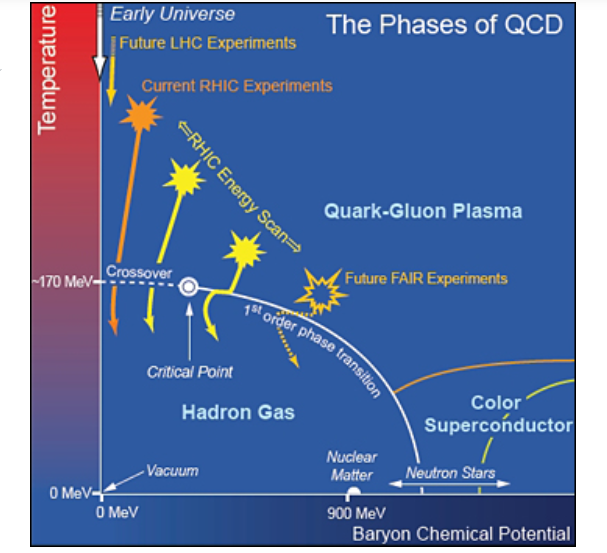
\includegraphics[scale=0.7]{STAR_results/QCD_phase_diagram}
		\caption{Διάγραμμα Φάσης Θερμοκρασίας, Θερμοκρασία συναρτήσει του χημικού δυναμικού των βαρυονίων. Η χρήση της πυκνότητας του χημικού δυναμικού για τον βαρυονικό αριθμό θα έδινε αντίστοιχο διάγραμμα φάσεων. Αυτό μπορούμε να το δούμε διαισθητικά αν θεωρήσουμε το σύστημα ως ένα αέριο φερμιονίων. Εκεί έχουμε ότι $\mu\sim E_f \sim p_F^2 \sim   density^{2/3}$}
		\label{fig4.3}
	\end{figure}
	
	
	Αριθμητικοί υπολογισμοί στην LQCD(Lattice QCD) έχουν δώσει αποτελέσματα τα οποία δίνουν αλλαγή φάσης για μηδενικό βαρυονικό χημικό δυναμικό σε θερμοκρασία περίπου 170MeV. Για παράδειγμα στην Εικόνα (\ref{fig4.4}) φαίνεται πως περίπου σε αυτή την θερμοκρασία υπάρχει έντονη μεταβολή του μεγέθους $P/T^4$ το οποίο έρχεται σε κορεσμό περίπου στην διπλάσια θερμοκρασία για διάφορες παραδοχές για τις γεύσεις των κουάρκ. Φαίνεται επίσης η σύγκριση των εν λόγω υπολογισμών με τα αποτελέσματα της σχεσης (\ref{eq4.1}). Αυτή η διαφορά υποδεικνύει πως οι αλληλεπιδράσεις και η μάζα των κουάρκ έχουν σημαντικό ρόλο στην μελέτη, όπως είναι και το προφανές.
	
	
	\begin{figure}[h!]
		\centering
		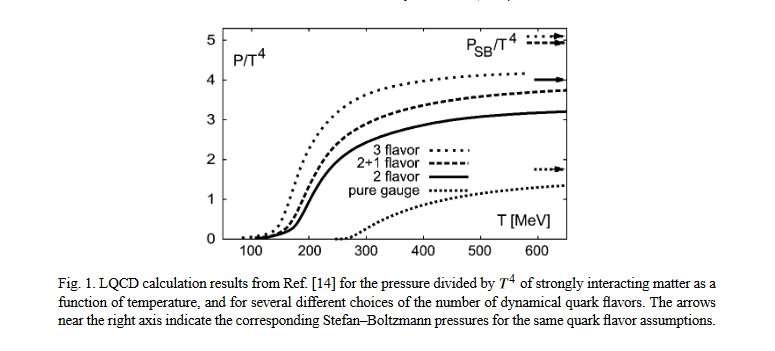
\includegraphics[scale=0.7]{STAR_Results/Predictions/P_over_T4_diagaram}
		\caption{Διάγραμμα πίεσης ανά $T^4$ συναρτήσει της θερμοκρασίας που έχει προκύψει από υπολογισμούς στην LWQCD και στο οποίο φαίνεται η πιθανή αλλαγή φάση  σε θερμοκρασία ~170MeV}
		\label{fig4.4}
	\end{figure}
	
	%Υπάρχουν επίσης υδροδυναμικά μοντέλα τα οποία στοχεύουν στο να υπολογίσουν την κάθετη ροή των προϊόντνω της σκέδασης. Αυτά προβλέπουν πως αυτή η ροή θα έχει ελλειπτικό σχήμα και λειτουργούν επίσης σε καταστάσεις ισορροπίας μέσω καταστατικών εξισώσεων.
	%Ακόμη, τα στατιστικά μοντέλα περιγράφουν την μακροσκοπική συμπεριφορά της κατάστασης ισοροπίας, αλλά δεν περιγράφουν τον τρόπο με τον οποία επιτυγχάνεται.
\subsection{Μερικά από τα αποτελέσματα των πρώτων χρόνων λειτουργίας του STAR}	
	
	Οι μετρήσεις των τελικών αδρονίων από τις συγκρούσεις βαρέων ιόντων αποκάλυψαν πως υπάρχουν τρεις διακριτές περιοχές της κάθετης στην δέσμη ορμής όπου έχουμε διαφορετική συμποεριφορά. Η "\textit{soft range}" $p_T\leq 1.5GeV/c$ η οποία περιέχει και το μεγαλύτερο πλήθος αδρονίων, η "\textit{hard-scattering range}" με $p_T\geq 6GeV/c$ η οποία παρέχει αποτελέσματα για τις καταστάσεις των παρτονίων στα πρώτα στάδια των κρούσεων. Ακόμη υπάρχει και η ενδιάμεση περιοχή "\textit{intermediate range}", με $1.5\leq p_T\leq 6GeV/c$ όπου περιέχονται ταυτόχρονα διαδικασίες και καταστάσεις και από τις προηγούμενες δύο περοχές. 	
	
	Αρχικά στην \textit{soft} περιοχή έχει παρατηρηθεί πως η ύλη που παράγεται παρουσιάζει συλλογική ροή\footnote{Η ροή εδώ αναφέρεται στην εξάρτηση της ενέργειας, της ορμής και της αριθμητικής πυκνότητας των σωματιδίων από την κατεύθυνση.}. 
	Γενικά, υπάρχει ένα μέτρο της μη ισοτροπικής ροής προς όλες της κατευθύνσεις το οποίο λέγεται \textit{elliptic flow}. Συγκεκριμένα περιγράφει την ανισοτροπικότητα της ροής στην αζιμουθιακή διεύθυνση $\phi$ σε ένα επίπεδο κάθετο στην δέσμη. 
	%Ορίζεται ως ο δεύτερος συντελεστής Fourier, από το ανάπτυγμα σε τριγωνομετρική σειρά Fourier της συνάρτησης $d^3N/d^3\bm{p}$, όπου $\bm{p}$ η ορμή ενός σωματιδίου, και Ν ο αριθμός των αλληλεπιδρώντων σωματιδίων και προκύπτει ότι είναι 
%	\begin{align*}\label{eq4.2}	
%		u_2 (p_t,y)=\braket{cos(2[(\phi-\Psi_{RP}])} \numberthis
%	\end{align*}
%	όπου $\phi$ είναι η αζιμουθιακή γωνία και $\Psi_{RP}$ είναι η γωνία του  επιπέδου που σχηματίζει το διάνυσμα της κατεύθυνσης της δέσμης με το διάνυσμα παραμέτρου κρούσης που ενώνει τα κέντρα των δύο ιόντων με  τον άξονα.
	
	Όταν τα τα προϊόντα της κρούσης έρθουν σε χαμηλότερη θερμοκρασία, τότε η ορμή των σωματιδίων μεταφέρεται στα τελικά αδρόνια που σχηματίζονται. Αυτά είναι που ανιχνεύουμε και ο ροή των οποίων μπορεί να μας οδηγήσει σε συμπεράσματα για την πρώτερη κατάσταση και η ανισοτροπικότητά της αποτελεί ένδειξη για την δημιουργία του QGP.
	Η αζιμουθιακή κατανομή των σωματιδίων είναι περιοδική συνάρτηση του $\phi$ και γράφεται ως σειρά Fourier. 
	\begin{align*}\label{eq4.2}
		f(\phi) = \frac{\alpha_0}{2\pi} + \frac{1}{\pi} \left( \sum_{n=1}^\infty \alpha_n cos(n\phi) + b_n sin(n\phi)\right) \numberthis
	\end{align*}
	%
	Όπου $\alpha_n$, $b_n$ οι συνηθισμένοι συντελεστές Fourier με $\alpha_0=N$. Αν θέσουμε $-\pi/n < \psi_n < \pi/n$ και $\omega_n =\sqrt{\alpha_n^2+b_n^2}$ τότε γίνεται 
	\begin{align*}\label{eq4.3}
		f(\phi) = \frac{N}{2\pi}\left( 1 + \sum_{n=1}^\infty 2\underbrace{\frac{\omega_n}{\omega_0}}_{v_n}cos(n(\phi-\psi_n) )\right) \numberthis
	\end{align*}
 Όπου οι συντελεστές ροής $v_n$ που σχετίζονται με το σχήμα και την ανισοτροπικότητα της ροής δίνονται από την σχέση 
 	\begin{align*}\label{eq4.4}
 		v_n = \braket{ cos(n(\phi-\psi_n))} \numberthis
 	\end{align*}
 	
 	Ενδεικτικά ο συντελεστής $v_2$ ονομάζεται \textit{elliptical flow} και αναπαριστά την εκκεντρότητα της ελλειψοειδώς ανισοτροπικής ροής που προκύπτει από μία \textit{peripheral} συγκρουση.
 
	Τα τελικά αδρόνια στην \textit{soft} περιοχή φαίνεται να ακολουθούν μία κίνηση υπό ένα κοινό, κάθετο στην δέσμη, πεδίο ταχυτήτων που επηρεάζεται από τις συνθήκες που επικρατούσαν στην αρχή της σκέδασης όπου είχαμε γρήγορη διαστολή των προϊόντνω υπό ένα μη ισοτροπικό πεδίο πίεσης και συχνές αλληλεπιδράσεις.
	Η συλλογικότητα της ροής φαίνεται από την εξάρτηση του συντελεστή \textit{elliptic flow} από την μάζα των τελικών αδρονίων σε χαμηλή $p_T$, Εικόνα (\ref{fig4.5}). Τα πειραματικά δεδομένα φαίνεται να συμπίπτουν με τους υδροδυναμικούς υπολογισμούς που υποθέτουν σύντομη θερμοποίηση, εκτόνωση σαν ιδανικό αέριο, αλλαγή φάσης σε θερμοκρασία περίπου 170MeV. 

\begin{figure}[h!]
	\centering
	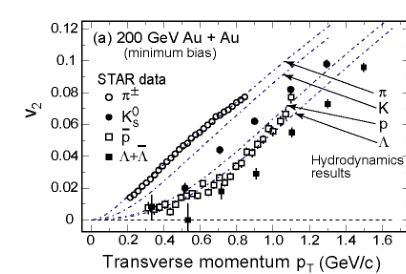
\includegraphics[scale=0.8]{STAR_Results/result_soft_1}
	\caption{Εξάρτηση του συντελεστή $v_2$ από την ορμή $p_T$ σε συγκρούσεις 200GeV/n Au-Au. Φαίνεται έτσι η συλλογική ροή των παραγόμενων σωματιδίων. }
	\label{fig4.5}
\end{figure}

	Ένα άλλο αποτέλεσμα είναι ότι οι περισσότερες ιδιότητες του κύριου όγκου που μετρήθηκαν φαίνονται παρόμοιες με αυτές που προέκυπταν από συγκρούσεις βαρέων ιόντων σε χαμηλότερες ενέργειες (ενδεικτικά αποτελέσματα στις Εικόνες (\ref{fig4.6}) \& (\ref{fig4.7})).
	 Πριν από τα αποτλέσματα του STAR οι θεωρητικές προβλέψεις πρότειναν ισχυρή εξάρτηση των εν  λόγωιδιοτήτων από την ενέργεια.
	Η παρατηρούμενη ομαλή συμπεριφορά των ιδιοτήτων αρχικά αποδόθηκε στο ότι το QGP  δημιουργείται από ένα εύρος αρχικών τοπικών συνθηκών, ακόμη και για δεδομένη ενέργεια και παράμετρο κρούσης.
	Στην Εικόνα (\ref{fig4.6}) παρατηρούμε πως η εξάρτηση του συντελεστή $v_2$ \textit{elliptical flow} από την ενέργεια, στην \textit{soft} περιοχή των συγκρούσεων υψηλής ενέργειας, είναι κοντά με την εξάρτηση του αντίστοιχου συντελεστή των συγκρούσεων χαμηλότερης ενέργειας.
	Στην Εικόνα (\ref{fig4.7}) φαίνεται η συνδιασπορά στην ορμή $p_T$ φορτισμένων σωματιδίων συναρτήσει του αριθμού των σωματιδίων $N_{part}$ που λαμβάνουν μέρος στην κρούση από την οποίο εξαρτάται η κεντρικότητα.
	%
	Η κεντρικότητα (centrality) ορίζεται ως το ποσοστό της ενεργού διατομής από ένα κατώφλι σωματδίων ως προς την συνολική ενεργό διατομή  
	\begin{align*}\label{eq4.5}
			%c(b) = \frac{\pi b^2}{\sigma_{inel}}  
			c = \frac{1}{\sigma_{AA}}\int_{N_{ch}^{thresh}}^{\infty} \odv{\sigma}{N_ch}'dN_{ch}' \propto \frac{1}{N_{part}}\numberthis
		\end{align*}	
	όπου b η παράμετρος κρούσης, δηλαδή η απόσταση των κέντρων των δύο πυρήνων και $\sigma_{inel}$ η συνολική ενεργός διατομή της σκέδασης. Πρόκεται για ένα μέτρο του πόσο κεντρική είναι η κρούση.
	
	
	\begin{figure}[h!]
	    \centering
	    \begin{minipage}{.5\textwidth}
	        \centering
	        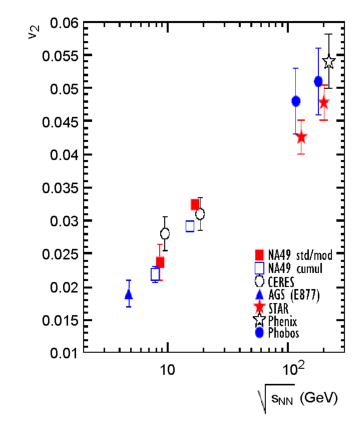
\includegraphics[scale=0.7]{STAR_Results/energy_dependence_of_v2}
	        \caption{Εξάρτηση του συντελεστή \textit{ellipitic flow} από την ενέργεια}
	        \label{fig4.6}
	    \end{minipage}%
	    \begin{minipage}{0.5\textwidth}
	        \centering
	        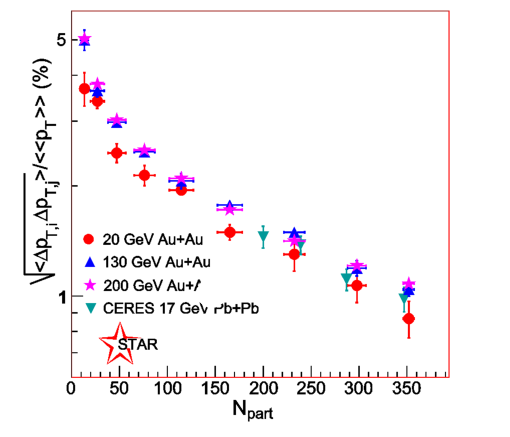
\includegraphics[scale=0.7]{STAR_Results/momentum_covariance_4_charged_particle_pairs}
	        \caption{Εξάρτηση της ρίζας της συνδιασποράς για ζεύγη φορτισμένων σωματιδίων  (προς την $p_T$) από την κεντρικότητα για διάφορες τιμές ενεργειών}
	        \label{fig4.7}
	    \end{minipage}
	\end{figure}
	
	
%	Ένα τελευταίο αποτέλεσμα σχετικό με την \textit{soft} περιοχή είναι η παραγωγή διαφορετικών ειδών, έως και strange, βαρυονίων γίνεται συνεπής με την Μεγαλοκανονική Κατανομή σε με
%	
%\begin{figure}[h!]
%	\centering
%	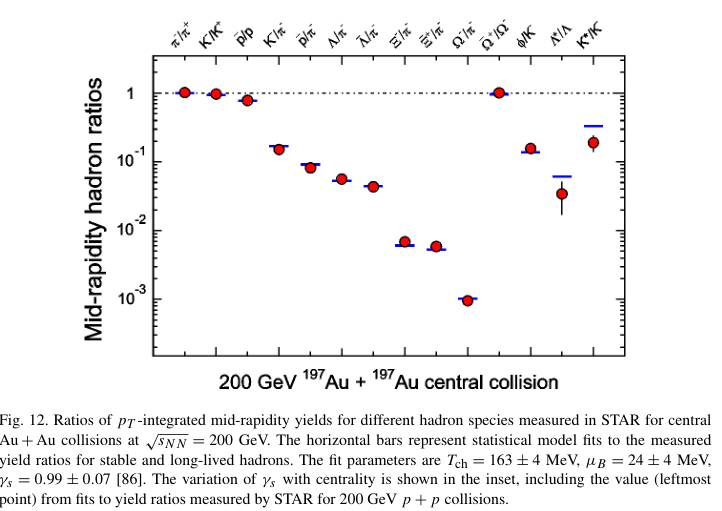
\includegraphics[scale=0.7]{STAR_Results/results_good_statistical1}
%	\caption{Προβλέψεις της στατιστικής θεωρίας για την λόγο διάφορων αδρονίων (μπλέ γραμμές) σε σύγκριση με τα περιαμταικά αποτελέσματα σε συγκρούσεις 200GeV}
%	\label{fig4.8}
%\end{figure}

	Σχετικά με την  \textit{intermediate} $p_T$ περιοχή.
Εδώ επέρχεται κορεσμός του \textit{elliptic flow, $v_2$}, δηλαδή η ροή τείνει προς την ισοτροπική (Εικονα (\ref{fig4.8})) και βλέπουμε διαφορές στην πυκνότητα και την $v_2$ βαρυονίων-μεσονίων. 
	Για παράδειγμα στην Εικόνα (\ref{fig4.9}) βλέπουμε το $R_{CP}$ συναρτήσει της $p_T$. Το $R_{CP}$ σχετίζεται με τον λόγο των κεντρικών συγκρούσεων (b=0) προς των peripheral συγκρούσεων ($0<b<R_1+R_2$). Εκεί βλέπουμε ότι ο λόγος $R_{CP}$ δεν σχετίζεται με την μάζα των βαρυονίων/μεσονίων αλλά σχετίζεται με τον άν πρόκειται για βαρυόνιο η μεσόνιο. 
	

		
		\begin{figure}[h!]
		    \centering
		    \begin{minipage}{.5\textwidth}
		        \centering
		        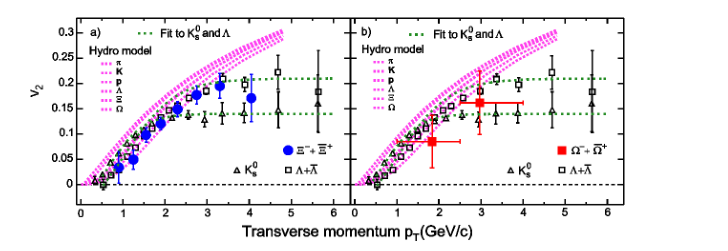
\includegraphics[width=1.1\linewidth, height=0.2\textheight]{STAR_Results/results_intermediate}
		        \caption{Κορεσμός του \textit{elliptical flow} στην intermediate περιοχή}
		        \label{fig4.8}
		    \end{minipage}%
		    \begin{minipage}{0.5\textwidth}
		        \centering
		        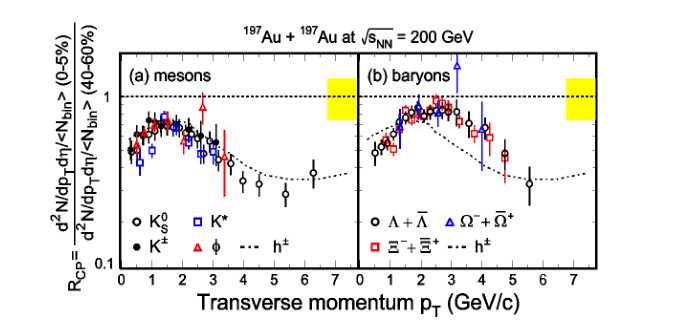
\includegraphics[width=1.1\linewidth, height=0.2\textheight]{STAR_Results/results_intermediate2}
		        \caption{Λόγος κεντρικών προς peripheral συγκρούσεων για μεσόνια και βαρυόνια συναρτήσει της $p_T$}
		        \label{fig4.9}
		    \end{minipage}
		\end{figure}   
	
	Ακόμη, υπήρχε άλλη μία ένδειξη πως στην δημιουργία του QGP ευνοοείται ο σχηματισμός \textit{strange} αδρνίων, δηλαδή αδρονίων που περιλαμβάνουν ένα τουλάχιστον \textit{strange } κουάρκ. Στις συνήθεις αδρονικές αντιδράσεις η παραγωγή των \textit{strange} κουάρκ καταπιέζεται εξαιτίας της μεγάλης τους μάζας ($m_s\simeq 95MeV/c^2$ ) σε σύγκριση με τα \textit{up} και \textit{down} ($m_u\simeq2.2MeV/c^2, m_d\simeq4.7MeV/c^2$). 
	Όμως στην φάση που δημιουργείται το QGP η θερμοκρασία που επικρατεί ευνοεί την παραγωγή \textit{strange} κουάρκ  και κατ' επέκταση ζεύγων $s\bar{s}$. Αυτό γίνεται αντιληπτό από την παραγωγή βαρυονίων και μεσονίων που περιέχουν $s$ ή $\bar{s}$. 
	Δεδομένου οτι τα Καόνια αποτελούνται από ένα \textit{strange} αντικουάρκ ($K^+(u\bar{s}), K^0(d\bar{s})$) και τα Πιόνια μόνο από \textit{up \& down} κουάρκ    ($\pi^+(u\bar{d}), \pi^0(u\bar{u},d\bar{d})$), αν μετρήσουμε τον λόγο παραγωγής τους, τότε θα δούμε ότι υπάρχει όντως μία αυξημένη παρουσία των Καονίων στην φάση του QGP στην περιοχή μέσης rapidity, άρα και μέσης ορμής. Αυτά τα αποτελέσματα του STAR φαίνονται στην Εικόνα (\ref{fig4.10}) όπου η παραγωγή s κουάρκ ευνοείται στις συγκρούσεις Au-Au έναντι των p-p.
	
	\begin{figure}[h!]
		\centering
		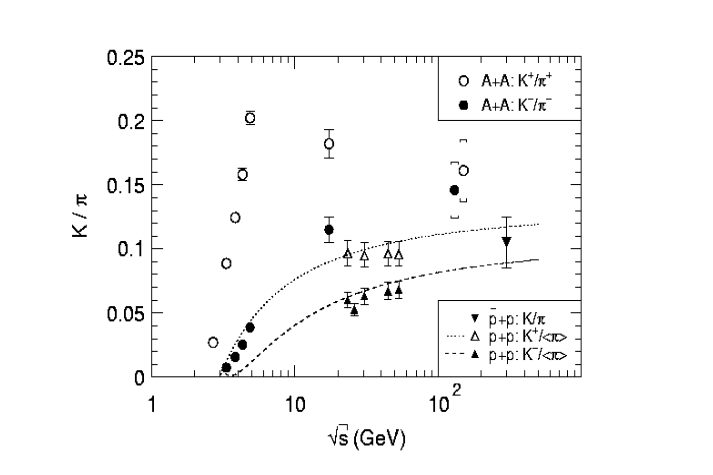
\includegraphics[scale=0.7]{STAR_Results/strange_enhancement}
		\caption{Λόγος της παραγωγής Κ/$\pi$ συναρτήσει της ορμής}
		\label{fig4.10}
	\end{figure}
	
%%%%%%%%%%%%%%%%%%%%%%%  HARD SECTOR	%%%%%%%%%%%%%%%%%%%%%%
		Τέλος, σχετικά με την \textit{hard} περιοχή. 
	%Το κύριο χαρακτηριστικό εκεί είναι ο κορεσμός σε υψηλό επίπεδο της \textcolor{red}{κατάπνιξης} (\textiit{suppression}) των αδρονίων , συγκριτικά με τις αναμενόμενες από άλλες συγκρούσεις p-p, peripheral Au-Au. \textit{Suppression} αδρονίων είναι όταν τα αδρόνια παράγονται σε χαμηλό ποσοστό από τα 
	Το κύριο χαρακτηριστικό είναι η ισχυρή καταπίεση (suppression) της παραγωγής αδρονίων και μεσονίων όπως το J/$\psi$ σε κεντρικές  συγκρούσεις Au-Au, το οποίο θεωρείται ως ένδειξη για την δημιουργία του QGP. Καθώς τα κουάρκ και τα αντικουάρκ αποδεσμεύονται από τα αδρόνια και τα μεσόνια δημιουργείται χωρικό φορτίο χρώματος και κατ'επέκταση μία θωράκιση της ισχυρής πυρηνικής δύναμης κάπως ανάλογα με την θωράκιση Debye στα αέρια ελεύθερων ηλεκτρονίων. Τότε, αυτή η θωράκιση εμποδίζει την δημιουργία καταστάσεων με πολλά κουάρκ καθώς μειώνεται η μεταξύ τους αλληλεπίδραση.
	%Experimenta and theoretical... pg 167 2nd bullet
	
\begin{figure}[h!]
	\centering
	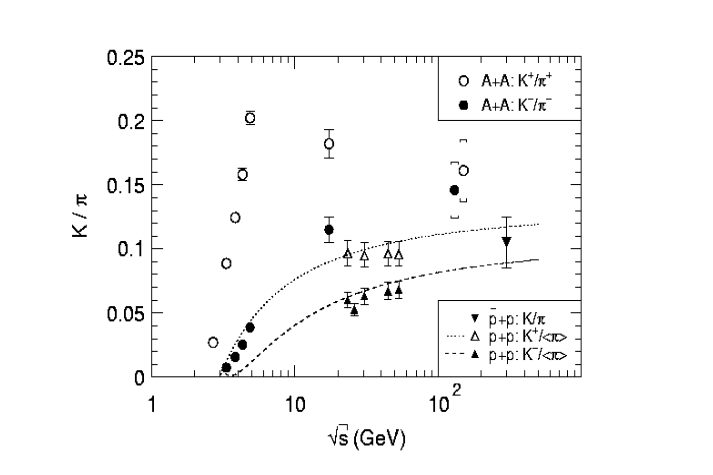
\includegraphics[scale=0]{STAR_Results/strange_enhancement}
	\textcolor{white}{\caption{Μέιωση της παραγωγής αδρονίων όσο αυξάνεται η ορμή $p_T$}}
	\label{fig4.11}
\end{figure}

	Μία ακόμη ένδειξη για την δημιουργία του QGP που προέρχεται από την περιοχή υψηλών ορμών είναι η το φαινόμενο \textit{jet quenching}. 
	Οι ισχυρές συγκρούσεις παρτονίων οδηγούν σε παραγωγή κουάρκ και γλουονίων με μεγάλη ορμή τα οποία διαχωρίζονται σε έναν μεγάλο αριθμό από ισχρά κατευθυνόμενα αδρονια, τα jets. 
	Τα jets, δημιουργούνται σε αρχικά στάδια της σύγκρουσης των βαρέων ιόντων πολύ πριν την δημιουργία της πυκνής ύλης. Τα jet θα "αισθανθούν" την πλήρη εξέλιξη της σύγκρουσης και έτσι θα φέρουν πληροφορίες και από την φάση όπου δημιουργείται η πυκνή και θερμή ύλη. Επειδή η πλειοψηφία των ισχυρών συγκρούσεων είναι μεταξύ δύο σωμάτων, θα παρατηρούμε δύο jets. Σε συγκρούσεις Au-Au,  υπάρχει η πιθανότητα τα jets να γεννηθούν κοντά στην δημιουργία του QGP. Τότε το ένα απ' τα δύο jets κάποιου γεγονότος θα εκπεμφθεί προς την μία μερία, απομακρυνόμενο από το QGP, ενώ το άλλο θα περάσει αναγκστικά από το εσωτερικό του QGP.
	Τώρα, αν όντως το QGP υπάρχει, τότε τα παρτόνια του jet που περνάει από το εσωτερικό του μπορεί να χάσουν τόση ενέργεια ώστε να μην προλάβουν να δημιουργηθούν αδρόνια. Αυτό το φαινόμενο είναι το \textit{jet quenching}.
	
	Για να μετρηθεί το \textit{jet quenching} σε πειράματα βαρέων ιόντων, πρέπει να χρησιμοποιηθεί η συσχέτιση (correlation) ανάμεσα σε δύο αδρόνια υψηλής ορμής.
	Αν μετρηθεί ένα τέτοιο αδρόνιο, που υποθέτουμε ότι προέρχεται από jet, τότε θα πρέπει να μετρηθεί και άλλο ένα με διαφορά αζιμουθιακης γωνίας $\Delta\phi=\pi$. Αν δεν μετρηθεί τότε θεωρούμε πως το δεύτερο jet έχει διέλθει εντός του QGP και έχει καταπνιχθεί. 
	Αυτό φαίνεται στην Εικόνα (\ref{fig4.12}) όπου σε συγκρούσεις d-Au \& p-p  παρατηρείται και δεύτερο jet, ενώ σε συγκρούσεις Au-Au δεν παρατηρείται και έτσι θεωρούμε πως εκεί δημιουργείται QGP.
	
	\begin{figure}[h!]
		\centering
		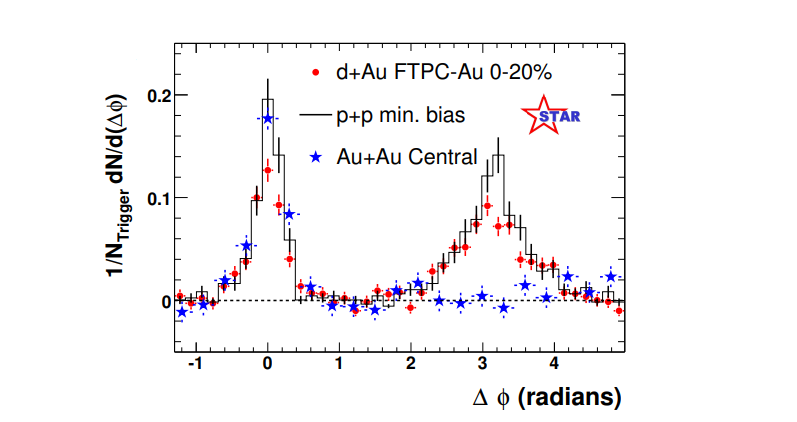
\includegraphics[scale=0.9]{STAR_Results/jet_quenching}
		\caption{Το δεύτερο jet αδρονίου δεν παρατηρείται σε γωνία π από το πρώτο}
		\label{fig4.12}
	\end{figure}
	
	
	\subsection{Γενικότερα Αποτελέσματα}	
		\subsubsection{Πρώτη Παρατήρηση του (anti-)Hypertriton }
						
		Ένα μικρό, αλλά σημαντικό, ποσοστό των παραγόμενων σωματιδίων μία σύγκρουσης βαρέων ιόντων αποτελούν και οι ελαφρείς πυρήνες. Παρατηρήθηκαν $70\pm17$ anti-hypertriton και $157\pm30$ hypertriton πυρήνες, με τους πρώτους να παρατηρθούνται για πρώτη φορά στο STAR έπειτα από συγκρούσεις Au-Au. Ο anti-hypertriton  πυρήνας αποτελείται από αντιπρωτόνιο, αντινετρόνιο και ένα αντι-Λαμδα ($\Lambda$). Η μελέτη των χαρακτηριστικών του παραπάνω ζεύγους πυρήνα-αντιπυρήνα μπορεί να οδηγήσει σε έλεγχο της συμμετρίας CPT για την οποία μέχρι στιγμής δεν έχει βρεθεί κάποια παραβίαση. 
			
			Επειδή ο εν λόγω πυρήνας είναι πολύ ασταθής δεν μπορεί να ανιχνευθεί ευθέως και γι'αυτό ανιχνεύουμε τα προίόντα των διασπάσεών του $^3_{\bar{\Lambda}}\bar{H}\rightarrow ^3\bar{He}+ \pi^+$ 
			%η οποία έχει πιθανότηα 25\% να συμβεί. 
	και $^3_\Lambda H\rightarrow d+p+\pi^-$.
			Τα  παραγόμενα σωματίδια κινούνται στον TPC μεταξύ εκατοντάδων άλλων φορτισμένων σωματιδίων όπως φαίνεται στην Εικόνα (\ref{fig4.12}) όπου έχουν ανακατασκευαστεί οι τροχιές των τελικών σωματιδίων της κρούσης.
		Μετρήθηκε η μάζα του πυρήνα και του αντίστοιχου αντι-πυρήνα χωρίς διαφορά στα πλαίσια των σφαλμάτων $m(^3_\Lambda H)=2.989\pm0.001\pm0.002GeV/c^2$ και $m(^3_{\bar{\Lambda}} \bar{H} ) = 2.991\pm0.001\pm0.002GeV/c^2$. Το δεύτερο σφάλμα των 2MeV/$c^2$ πρόκειται για το συστηματικό σφάλμα που προκύπτει από τις μικρές αποκλίσεις των τροχιών των προϊόντων της διάσπασης εντός του TPC, από τις ιδανικές.
		Μετρήθηκε ακόμη ο χρόνος ζωής των παραπάνω πυρήνων και πάλι όπως είναι αναμενόμενο από την συμμετρία ύλης-αντιύλης δεν βρέθηκε να διαφέρουν στα όρια του σφάλματός τους $\tau = 182\pm27ps$.
		Οι μετρήσεις του χρούνου ζωής δεν συμφωνούν με άλλα πειράματα , με αποτέλεσμα να μην είναι εφικτή η επιλογή κάποιου θεωρητικού μοντέλου για την περιγραφή του συστήματος, παρά μόνο με φαινομενολογικούς υπολογισμούς που βασίζονται σε ansatz κυματοσυναρτήσεις η προσεγγίσεις, ως πρόβλημα τριών σωμάτων
			
			\begin{figure}[h!]
				\centering
				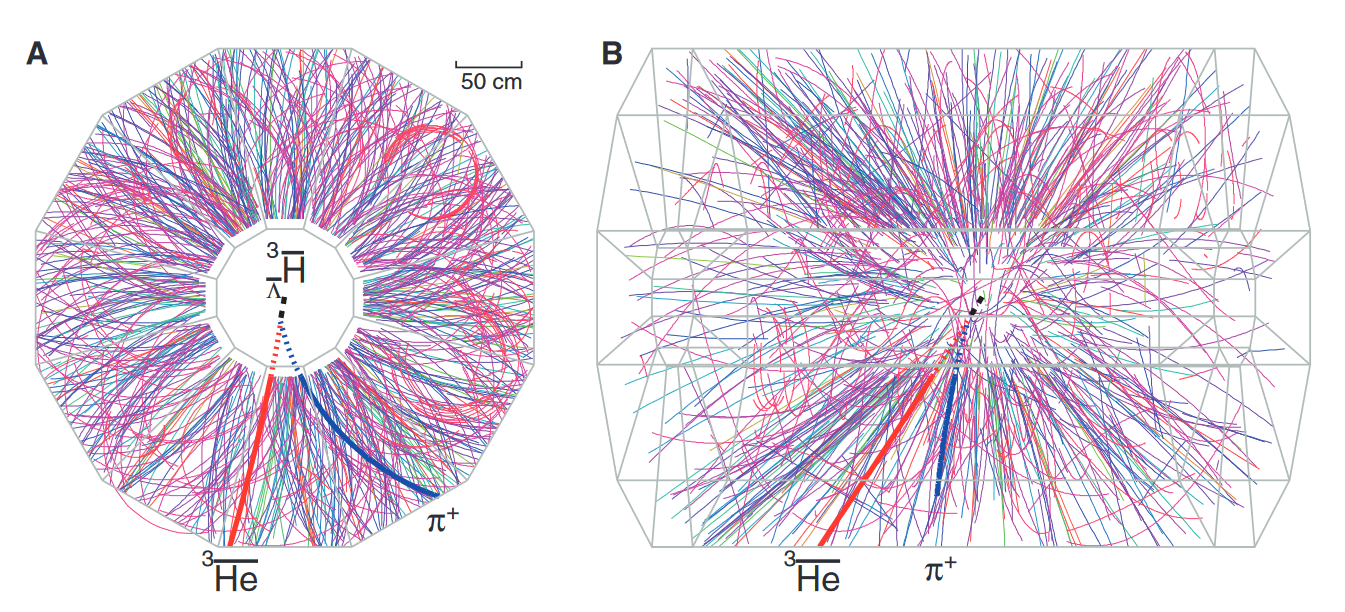
\includegraphics[scale=0.5]{STAR_Results/hypertriton_traj}
				\caption{Τοχιές των $ ^3\bar{He}, \pi^+$ μεταξύ των τροχιών όλων των υπόλοιπων σωματιδίων }
				\label{fig4.13}
			\end{figure}
			
	%%%% Βinding Energy 
	% TOF, TPC, HFT , SSD 
Τέλος, μετρήθηκε η ενέργεια σύνδεσης, $B_\Lambda$ του hypertriton, η οποία βάσει των παραπάνω αποτελεσμάτων μη παραβίασης της CPT θεωρήθηκε ότι είναι ίδια με την ενέργεια σύνδεση τους anti-hypertriton. H $B_\Lambda$ υπολογίστηκε από την σχέση $B_\Lambda = (m_d+m_\Lambda -m_{^3_{\Lambda}H})c^2$, 
όπου για $m_{^3_{\Lambda}H}$ χρησιμοποιήθηκε ένας σταθμισμένος μέσος όρος των μαζών των $^3_{\Lambda}H, ^3_{\Lambda}\bar{H}$ που ισούται με $m=2.990\pm(stat)\pm0.11(syst)MeV/c^2$ και
 βρέθηκε ότι είναι $B_\Lambda=0.41\pm0.12(stat)\pm0.11(syst) MeV$. Στην παρακάτω Εικόνα (\ref{fig4.14}) φαίνεται η σύγκρισή της με άλλες μετρήσεις και θεωρητικούς υπολογισμούς.

\begin{figure}[h!]
		\centering
		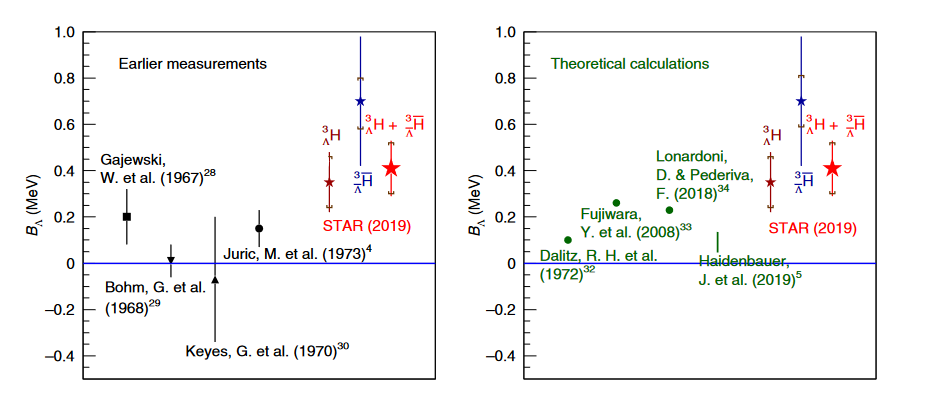
\includegraphics[scale=0.6]{STAR_Results/hypertriton_binding}
		\caption{Ενέργεια σύνδεσης του Hypertriton σε σύγκριση με παλαιότερες μετρήσεις και θεωρητικούς υπολογισμούς.}
		\label{fig4.14}
	\end{figure}
		
	
\section{Συγκρούσεις Πρωτονίων}

	Ένας από τους κύριους στόχους του προγράμματος συγκρούσεων πολωμένων πρωτονίων του RHIC, είναι να προσδιοριστεί η δομή του σπιν των νουκλεονίων, δηλαδή να επεξηγηθεί η σχέση
	\begin{align*}\label{eq4.6}
		\frac{1}{2} = \frac{1}{2}\Delta\Sigma +\Delta G + L_{Q,G} \numberthis
	\end{align*}
όπου $\Delta \Sigma$ είναι η συνεισφορά της ελικότητας των κουάρκ και των αντικουάρκ στο συνολικό σπιν, το $\Delta G$ το αντίστοιχο για τα γλουόνια και τα $L_{Q,G}$ είναι η συνεισφορά της τροχιακής κίνησης των κουάρκ και των γλουονίων στο συνολικό σπιν.

	Το κίνητρο για την απάντηση τέτοιων ερωτήσεων προέρχεται από το γεγονός ότι στα χρόνια πριν τον RHIC υπήρχαν ενδείξεις πως η συνεισφορά των κουάρκ στο σπιν των νουκλεονίων ήταν μόλις περίπου 25\%, ενώ των γλουονίων $<20\%$. Το ερώτημα λοιπόν είναι τί είναι αυτό το οποίο συμπληρώνει το υπολοιπόμενο σπιν; 
	Οι πιθανές απαντήσεις ήταν να πηγάζει από το σπιν των γλουονίων και από την περιστροφική κίνηση των κουάρκ και των γλουονίων όπως φαίνεται στην εξίσωση (\ref{eq4.6}).

\subsection{Αποτελέσματα Ασυμμετριών}

Όπως έχει αναφερθεί, η σημασία της πόλωσης των δεσμών πρωτονίων έγκειται στο γεγονός ότι με αυτόν τον τρόπο μπορούν να αναδειχτούν ασυμμετρίες στις ενεργές διατομές διαφορων αντιδράσεων ανάλογα με την πόλωση.
	Ενδεικτικά, για την εγκάρσια πόλωση υπάρχει ο παράγοντας (\textit{Transverse Single Spin Asymmetry, TSSA)}
		\begin{align*}\label{eq4.7}
			A_N = \frac{d\sigma^{\uparrow} - d\sigma^{\downarrow}}{d\sigma^{\uparrow} + d\sigma^{\downarrow}} \numberthis
		\end{align*}
	
	που ποσοτικοποιεί την ασυμμετρία μεταξύ των ενεργών διατομών των συγκρούσεων  άνω και κάτω πολωμένων δεσμών με μία μη πολωμένη δέσμη.
	Στο διάγραμμα της Εικόνας (\ref{fig4.15}) φαίνεται η αύξηση του $A_N^{\pi^0}$, δηλαδή του συντελεστή \textit{TSSA} για ουδέτερα πιόνια $\pi^0$, καθώς αυξάνεται η μεταβλητή $x_F = x_{bjorken,1}-x_{bjorken,2}$ και η ίδια συμπεριφορά παρατηρείται και σε \textit{jets}, όπως φαίνεται στην Εικόνα (\ref{fig4.17}).
	    
	
	\begin{figure}[h!]
		\centering
		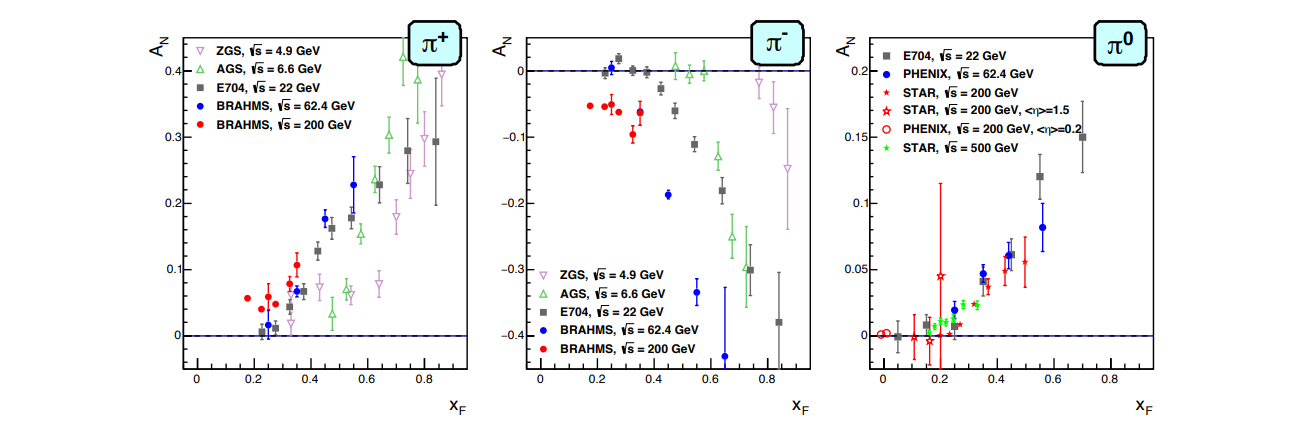
\includegraphics[scale=0.7]{STAR_Results/AN_pions_all}
	        \caption{Παράγοντας ασυμμετρίας των ενεργών διατομών για παραγωγή  πιονών ανάλογα με την αρχική εγκάρσια πόλωση συναρτήσει της μεταβλητής $x_F$}
		\label{fig4.15}
	\end{figure}
	
	
	\begin{figure}[h!]
			\centering
			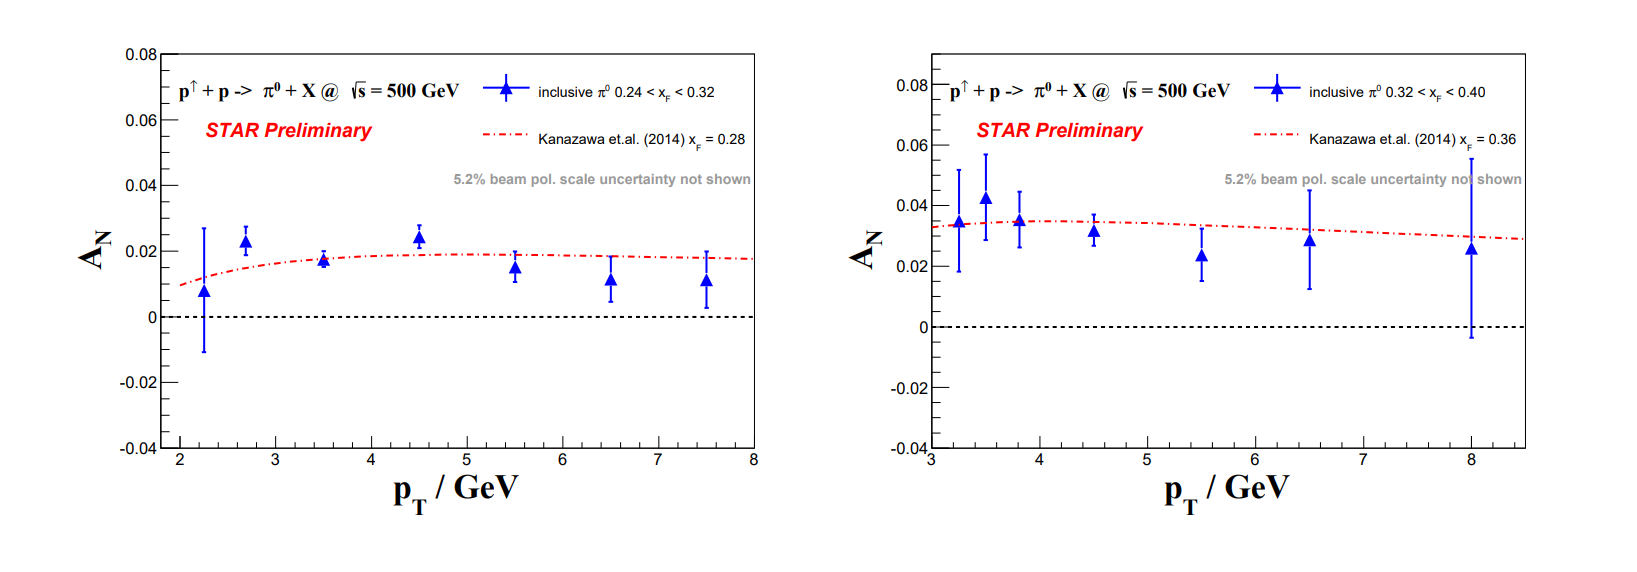
\includegraphics[scale=0.5]{STAR_Results/AN_pions_pt}
			\caption{Εξάρτηση του $A_N$ από την κάθετη ορμή $p_T$}
			\label{fig4.16}
		\end{figure}
			
	
	\begin{figure}[h!]
		\centering
		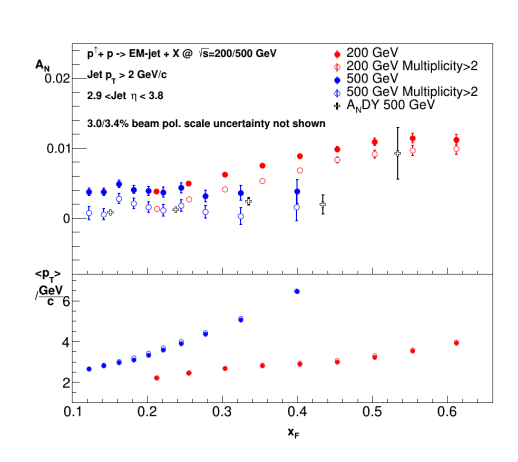
\includegraphics[scale=0.7]{STAR_Results/AN_jets}
	    \caption{Παράγοντας ασυμμετρίας των ενεργών διατομών για παραγωγή \textit{jet} συναρτήσει της $x_F$}
		\label{fig4.17}
	\end{figure}
	
	
	
	
 	Οι θεωρητικές ερμηνίες για τις παραπάνω ασυμμετρίες πηγάζουν από δύο διαφορετικές συναρτήσεις κατανομής του σπιν του πρωτονίου από τα παρτόνια (Parton Distribution Functions, PDFs) η μία κατηγορία εκ των οποίων έχει εξάρτηση από την ορμή $p_T$ και λέγεται TMD (Transverse Momentum Dependence PDF). 
 	Στην TMD, η συνάρτηση που πηγάζει από τον μηχανισμό που εισήγαγε ο Sivers περιγράφει την εγκάρσια κίνηση των παρτονίων σε ένα πολωμένο πρωτόνιο στην αρχική κατάσταση. Ο μηχανισμός Sivers, προτείνει πως η συνάρτηση κατανομής των κουάρκ (PDF) αποτελείται από δύο μέρη. Το πρώτο έχει να κάνει με το μη πολωμένο μέρος και το δεύτερο συζεύγνει την $p_T$ του κουάρκ με το σπιν του πρωτονίου.
 	Η συνάρτηση "σπασίματος" (fragmentation) Collins περιγράφει την πιθανότητα για ένα κουάρκ που είναι πολωμένο κάθετα στην ορμή να δημιουργήσει ένα πιόνιο που έχει ένα κομμάτι z από την ορμή του αρχικού κουάρκ. Αυτό σημαίνει πως η κατεύθυνση της αρχική πόλωσης καθορίζει την κατεύθυνση του παραγόμενου πιονίου.
 	
 	
	
	
	
	
	Αντίσοιχες ασυμμετρίες παρατηρούνται και όταν έχουμε διαμήκη πόλωση ως προς την κατεύθυνση της δέσμης. Ομοίως με πριν, ορίζουμε την \textit{single} και επιπλέον την \textit{double spin} ασυμμετρία.
		\begin{align*}\label{eq4.8}
			A_L    =& \frac{\sigma_+-\sigma_-}{\sigma_++\sigma_-} \numberthis \\
			A_{LL} =& \frac{\sigma^{++}+\sigma^{--} - \sigma^{+-}-\sigma^{-+}}{\sigma^{++}+\sigma^{--} + \sigma^{+-}+\sigma^{-+}} \numberthis
		\end{align*}
	
	Όπου $\sigma^\pm$ η ενεργός διατομή για τις διάφορες αντιδράσεις (π.χ. αντίστοιχα $\vec{p}p\rightarrow W^\pm X$) και οι $\sigma^{\bullet_1 \bullet_2}$ εκφράζουν τις ενεργές διατομές για τις διάφορες αντιδράσεις όταν η ελικότητα της μίας δέσμης είναι 	$\bullet_1$ και της άλλης $\bullet_2$.
	Στην Εικόνα (\ref{fig4.18}) φαίνεται η εξάρτηση του $A_L^{W^\pm}$ από την \textit{pseudorapidity} των ανιχνευόμενων ηλεκτρονίων, καθώς τα $W^\pm$ διασπώνται σε $e^\pm$.
	
	\begin{figure}[h!]
		\centering
		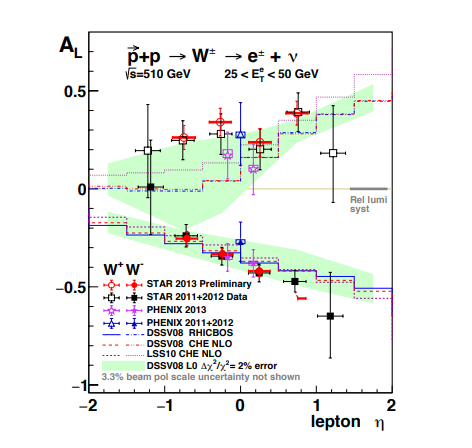
\includegraphics[scale=0.7]{STAR_Results/AL_parity_violation}
		\caption{Εξάρτηση του $A_L$ από την \textit{pseudorapidity} των τελικών ηλεκτρονίων από την οποία φαίνεται η παραβίαση της Parity}
		\label{fig4.18}
	\end{figure}
	
Στην Εικόνα (\ref{fig4.19}) φαίνεται η ασυμμετρία $A_{LL}$ που εμφανίζουν τα jet. 
	\begin{figure}[h!]
		\centering
		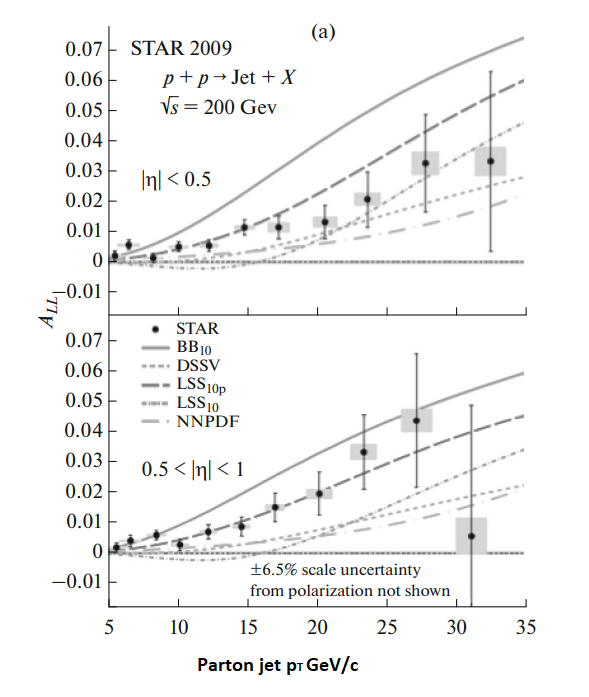
\includegraphics[scale=0.6]{STAR_Results/ALL_jet}
		\caption{Ασυμμετρία $A_{LL}^{jet}$ συναρτήσει της $p_T$ για συγκεκριμένες περιοχές \textit{pseudorapidity}}
		\label{fig4.19}
	\end{figure}
	
Στην Εικόνα (\ref{fig4.20}) φαίνεται πως στα όρια των πειραματικών σφαλμάτων η Parity διατηρείται στις αντιδράσεις $\vec{p}\vec{p}\rightarrow W^\pm X\rightarrow e^\pm+\nu+X$ όταν η δέσμη πρωτονίων είναι πολωμένη κατά μήκος της τροχιάς.	
	
	\begin{figure}[h!]
		\centering
		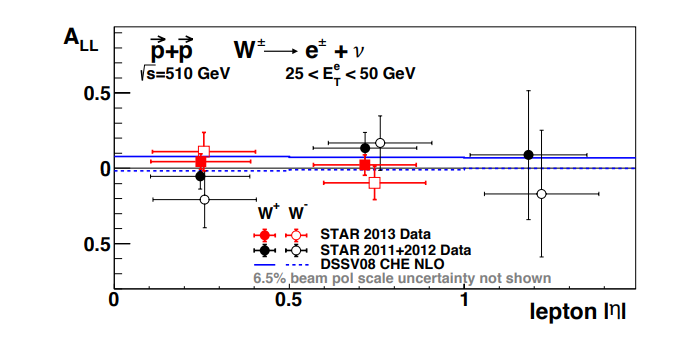
\includegraphics[scale=0.7]{STAR_Results/ALL_parity_conservation}
		\caption{$A_{LL}^{W^\pm}$ συναρτήσει της \textit{pseudorapidity} των τελικών ηλεκτρονίων όπου φαίνεται η διατήρηση της Parity}
		\label{fig4.20}
	\end{figure}
	
	